\hypertarget{a00017}{}\section{/\+Users/\+Kaden/\+Documents/project/\+Arc\+Syn3sis/3rd\+Party/parmetis-\/4.0.3/metis/\+G\+Klib/blas.c File Reference}
\label{a00017}\index{/\+Users/\+Kaden/\+Documents/project/\+Arc\+Syn3sis/3rd\+Party/parmetis-\/4.\+0.\+3/metis/\+G\+Klib/blas.\+c@{/\+Users/\+Kaden/\+Documents/project/\+Arc\+Syn3sis/3rd\+Party/parmetis-\/4.\+0.\+3/metis/\+G\+Klib/blas.\+c}}


This file contains G\+Klib\textquotesingle{}s implementation of B\+L\+A\+S-\/like routines.  


{\ttfamily \#include $<$G\+Klib.\+h$>$}\newline
Include dependency graph for blas.\+c\+:\nopagebreak
\begin{figure}[H]
\begin{center}
\leavevmode
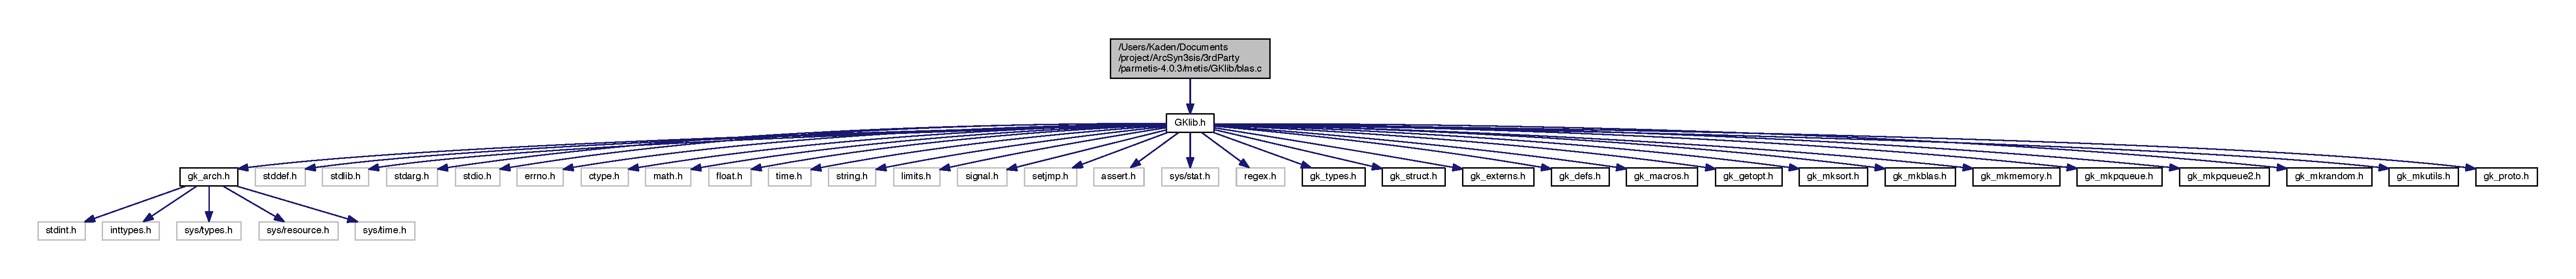
\includegraphics[width=350pt]{a00018}
\end{center}
\end{figure}


\subsection{Detailed Description}
This file contains G\+Klib\textquotesingle{}s implementation of B\+L\+A\+S-\/like routines. 

The B\+L\+AS routines that are currently implemented are mostly level-\/one. They follow a naming convention of the type gk\+\_\+\mbox{[}type\mbox{]}\mbox{[}name\mbox{]}, where \mbox{[}type\mbox{]} is one of c, i, f, and d, based on C\textquotesingle{}s four standard scalar datatypes of characters, integers, floats, and doubles.

These routines are implemented using a generic macro template, which is used for code generation.

\begin{DoxyDate}{Date}
Started 9/28/95 
\end{DoxyDate}
\begin{DoxyAuthor}{Author}
George 
\end{DoxyAuthor}
\begin{DoxyVersion}{Version}
\begin{DoxyVerb}$Id: blas.c 11848 2012-04-20 13:47:37Z karypis $ \end{DoxyVerb}
 
\end{DoxyVersion}
